\documentclass{article}
\usepackage{tikz}
\usetikzlibrary{external,shapes,calc,math,patterns,arrows,positioning,fadings}
\tikzexternalize[optimize=false]

\tikzstyle{node}=[circle, draw=black, minimum size=25pt, line width=1, inner sep= 5pt]
\tikzstyle{nodel}=[circle, draw=black, minimum size=15pt, line width=1, inner sep= 0pt]
\tikzstyle{tnode}=[nodel, minimum size=0.6 cm, fill=white]
\tikzstyle{node1}=[circle, draw=black, minimum size=15pt, line width=1, inner sep= 2pt]
\tikzstyle{node2}=[circle, draw=black, minimum size=8pt, line width=1, inner sep= 0pt, fill=white!70!black]
\tikzstyle{l1}=[line width=1]
\tikzfading[name=fade right, left color=transparent!0, right color=transparent!100]
\tikzstyle{odd}=[node1, dashed, pattern=dots, pattern color=mred!75!white]
\tikzstyle{even}=[node1, pattern=dots, pattern color=mblue!75!white]
\tikzstyle{lodd}=[odd, pattern = crosshatch dots]
\tikzstyle{leven}=[even, pattern = crosshatch dots]
\tikzstyle{enset}=[node1, thick, double, font=\footnotesize]
\tikzstyle{onset}=[node1, thick, densely dashed, double, font=\footnotesize]
\tikzstyle{subtree}=[node1, opacity=0.3,dotted, font=\footnotesize]

\usepackage{xcolor}
\definecolor{mblue}{HTML}{1F77B4}
\definecolor{morange}{HTML}{FF7F0E}
\definecolor{mgreen}{HTML}{2CA02C}
\definecolor{mred}{HTML}{D62728}
\definecolor{mpurple}{HTML}{9467BD}
\definecolor{mbrown}{HTML}{8C564B}
\definecolor{mpink}{HTML}{E377C2}
\definecolor{mgrey}{HTML}{7F7F7F}
\definecolor{mlime}{HTML}{BCBD22}
\definecolor{mcyan}{HTML}{17BECF}

\begin{document}
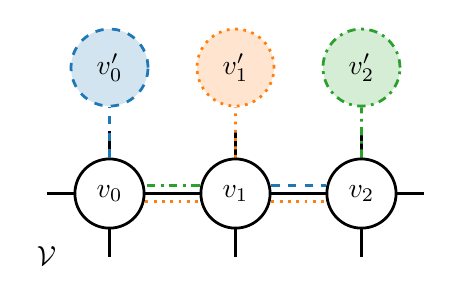
\begin{tikzpicture}[scale=0.8]

    \node at (-1, -1) {$\mathcal{V}$};
    \draw[l1] (0, 0) -- (4,0);
    \draw[l1] (-1,0) -- (5,0);
    \draw[l1] (0,1) -- (0,-1);
    \draw[l1] (2,1) -- (2,-1);
    \draw[l1] (4,1) -- (4,-1);
    \node[node, fill=white] at (0,0) (1) {$v_0$};
    \node[node, draw=mblue, fill=mblue, fill opacity=.2, text opacity=1, dashed] at (0,2) (2) {$v_0'$};
    \node[node, fill=white] at (2,0) (3){$v_1$};
    \node[node, draw=morange, fill=morange, fill opacity=.2, text opacity=1,dotted] at (2,2) (4) {$v_1'$};
    \node[node, fill=white] at (4,0) (5) {$v_2$};
    \node[node, draw=mgreen, fill=mgreen, fill opacity=.2, text opacity=1,dashdotted] at (4,2) (6) {$v_2'$};

    \draw[l1, dashed, mblue] (1) -- (2);
    \draw[l1, dashed, mblue, transform canvas={yshift=3pt}] (3) -- (5);
    \draw[l1, dotted, morange] (3) -- (4);
    \draw[l1, dotted, morange, transform canvas={yshift=-3pt}] (1) -- (3) -- (5);
    \draw[l1, dashdotted, mgreen] (5) -- (6);
    \draw[l1, dashdotted, mgreen, transform canvas={yshift=3pt}] (3) -- (1);

\end{tikzpicture}

\begin{tikzpicture}[scale=0.8]
    \path[pattern=dots, pattern color=mblue] (0,3) arc (90:225:1) arc (45:-135:.4142) arc (45:315:1) arc (135:-45:.4142) arc (135:405:1) arc (225:135:.4142) arc (-45:45:1) arc (225:135:.4142) arc (-45:90:1) -- cycle;
    \path[pattern=grid , pattern color=morange] (2,1) arc (90:450:1);
    \node[node, fill=white!70!mblue] at (0,0) (0) {$v_1$};
    \node[node, fill=white!70!morange] at (2,0) (1) {$v_2$};
    \node[node, fill=white!70!black, path fading=fade right] at (4,0) (5) {$v_3$};
    \node[node, fill=white] at (-2,0) (2) {$v_4$};
    \node[node, fill=white] at (0,2) (3) {$v_5$};
    \node[node, fill=white] at (0,-2) (4) {$v_6$};
    \draw[l1] (1) -- (0) -- (3);
    \draw[l1] (2) -- (0) -- (4);
    \draw[l1, dotted] (2, 1.5) -- (1) -- (2,-1.5);
    \draw[l1] (1) -- (5);
    \node at (-4, 0) {$\mathcal{V}_e$};

    \node at (-4, -4.5) {$\mathcal{N}_e$}; 
    \node[node, pattern=dots, pattern color=mblue] at (0,-4.5) (d) {$n_1$};
    \node[node, pattern=grid , pattern color=morange] at (2,-4.5) (e) {$n_2$};
    \node[node, fill=white!70!black, path fading=fade right] at (4,-4.5) (f) {$n_3$};
    \draw[l1] (d) -- (e) -- (f);
\end{tikzpicture}


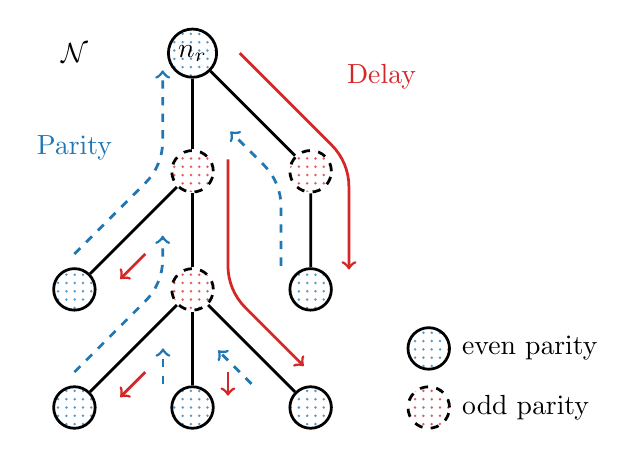
\begin{tikzpicture}[x=1.5cm,y=1.5cm]
    \node[node1,even] (a) at (1, 3) {$n_r$};
    \node[node1,odd]  (b) at (1, 2) {};
    \node[node1,odd]  (c) at (1, 1) {};
    \node[node1,even] (d) at (1, 0) {};
    \node[node1,even] (e) at (0, 1) {};
    \node[node1,even] (f) at (0, 0) {};
    \node[node1,odd]  (g) at (2, 2) {};
    \node[node1,even] (h) at (2, 1) {};
    \node[node1,even] (i) at (2, 0) {};
    \draw[l1] (a) -- (b) -- (c) -- (d);
    \draw[l1] (b) -- (e);
    \draw[l1] (c) -- (f);
    \draw[l1] (c) -- (i);
    \draw[l1] (a) -- (g) -- (h);

    \draw[l1, ->, dashed, color=mblue] (0, 1.3) -- +(45:0.85) arc (-45:0:.5) -- +(90:.6);
    \draw[l1, ->, dashed, color=mblue] (0, 0.3) -- +(45:0.85) arc (-45:0:.5) -- +(90:.2);
    \draw[l1, ->, dashed, color=mblue] (0.75,0.2) -- +(90:.3);
    \draw[l1, ->, dashed, color=mblue] (1.5,0.2) -- +(135:.4);
    \draw[l1, ->, dashed, color=mblue] (1.75,1.2) -- +(90:0.5) arc (0:45:.5) -- +(135:0.4);
    \draw[l1, ->, color=mred] (1.4, 3) -- +(-45:1.1) arc (45:0:0.5) -- +(-90:0.7);
    \draw[l1, ->, color=mred] (1.3, 2.1) -- +(-90:0.9) arc (180:225:.5) -- +(-45:0.7);
    \draw[l1, ->, color=mred] (0.6, 1.3) -- +(225:.3);
    \draw[l1, ->, color=mred] (0.6, 0.3) -- +(225:.3);
    \draw[l1, ->, color=mred] (1.3, 0.3) -- +(-90:.2);
    \node[text=mblue] at (0,2.2) {Parity};
    \node[text=mred] at (2.6,2.8) {Delay};
    \node at (0,3) {$\mathcal{N}$};

    \path (3,.5) node[node1, even]{} -- +(.2,0) node[anchor=west] {even parity}; 
    \path (3,0) node[node1, odd]{} -- +(.2,0) node[anchor=west] {odd parity}; 
\end{tikzpicture}
\end{document}